\documentclass[11pt]{article}

\usepackage{acl-style/acl}
\usepackage{times}
\usepackage{latexsym}
\usepackage[T1]{fontenc}
\usepackage[utf8]{inputenc}
\usepackage{microtype}
\usepackage{inconsolata}
\usepackage{amsmath}
\usepackage{amssymb}
\usepackage{booktabs}
\usepackage{graphicx}

\title{Better Judges, Same Answers:\\When Self-Verification Can and Cannot Improve Mathematical Reasoning}

\author{Aryama V Murthy \\ Mukund Hebbar \\ Yashas Nataraj Kotre \\ Anivarth Varma Penumetcha \\ IIIT Hyderabad}

\begin{document}
\maketitle

\begin{abstract}
Training a 2B model to judge its own mathematical attempts raised its AUROC from 0.57 to 0.67, yet picking among its
answers did not improve. We show this is predicted, not anomalous. Three measurement illusions hide what a
self-verifier can do:
(i) a lenient judge looks near chance under sampled verdicts even when its underlying score discriminates;
(ii) on a typical pool, 99.9\% of the pairs behind an AUROC compare different questions, while selection and repair
provably use only within-question information; and
(iii) majority vote saturates, and before that point verification cannot beat it at equal compute.

A five-parameter model fitted only to 4-attempt aggregates predicts the 16-attempt scaling curves of 16,000 new
attempts to within a point. Reading verdict probabilities instead of sampling verdicts raises the judge's AUROC by 0.07
to 0.09 (paired 95\% CIs exclude zero). Judge-free trace features match the trained judge's pooled AUROC yet are at
chance on contested questions, exactly as the theory requires.

The theory predicts a procedure, contest-adaptive verification, that spends judgement only where sampled answers
disagree. In a pre-registered test on 800 questions it beats majority vote at equal compute by $+1.6$ points
$[+0.5, +2.6]$ and passes the plateau that voting and adaptive-consistency share, close to the $\approx+1.3$ the
model predicted before judging.
\end{abstract}


\section{Introduction}
\label{sec:intro}

A model that can check its own work should be able to pick its best answer. We trained a 2B-parameter model,
Qwen3.5-2B, to judge its own mathematical attempts with answer-checker labels. Its AUROC on its own attempts rose from
$0.57$ to $0.67$, and the gain replicated on a held-out test set. Yet picking one of four answers with the trained
judge was no better than majority vote ($75.2\%$ either way), and flagging and regenerating attempts recovered $0.4$ of
the $7$ points that perfect flags would have recovered. Every off-the-shelf judge we tried looked ``near chance'' on
the model's own attempts.

We show that these outcomes are what the mathematics predicts. They come from three measurement illusions:
\begin{enumerate}
\item \textbf{Leniency.} A judge that almost always says ``correct'' has a near-chance AUROC under sampled verdicts,
  even when its underlying score discriminates (\S\ref{sec:lenient}).
\item \textbf{Pooled AUROC.} On a typical evaluation pool, $99.9\%$ of the pairs behind an AUROC compare
  \emph{different} questions. Picking and repair use only within-question information, exactly
  (Theorem~1, \S\ref{sec:pooled}).
\item \textbf{The compute regime.} Majority vote saturates. Verification cannot beat majority vote at equal compute
  before that point, and can after it (\S\ref{sec:scaling}).
\end{enumerate}

A model with five parameters reproduces the measured numbers, including three it was not fitted to
(Table~\ref{tab:validation}). It also predicts a simple procedure, \emph{contest-adaptive verification} (CAV), and a
training change (per-question balance), both of which we test on the model's own attempts
(\S\ref{sec:results}).

\paragraph{Contributions.}
\begin{itemize}
\item A calibrated model of self-verified answer selection.
\item An invariance theorem with an exact repair identity, a closed form for the gain from tie-breaking, and a
  saturation-and-consistency account of when verification pays.
\item Measurements of judge leniency and within-question discrimination on 16 own attempts per question.
\item CAV, evaluated against majority vote and adaptive-consistency at equal compute.
\item A proposition and an experiment on training judges for selection rather than for verdict accuracy.
\end{itemize}

\section{Setting}
\label{sec:setting}

\paragraph{Models and data.}
The solver and the judge are the same model: Qwen3.5-2B with a LoRA adapter trained by Dr.~GRPO \citep{liu2025drgrpo}
on equal thirds of three tasks: solving, judging injected errors, and reconstructing questions. Questions come from
DeepMath-103K \citep{he2026deepmath}: the 400-question test split, a 200-question development slice, and 400 held-out
training questions that the adapter never saw.

\paragraph{Protocol.}
For each question we sample 16 attempts (temperature $1.0$, 16k-token cap). Answers are graded by a rule-based checker.
The judge sees an attempt split into numbered steps and writes a verdict after optional reasoning (8k cap).

We read two scores:
\begin{itemize}
\item the probability of the verdict token after a reasoning chain;
\item a \emph{direct} probability, read right after the prompt with no reasoning \citep{kadavath2022know}.
\end{itemize}
Selection rules are averaged over 100 random orders of each question's attempts. Differences are bootstrapped over
questions \citep{miller2024errorbars}. The protocol was pre-registered before any attempt was generated
(\texttt{phase3/PREREGISTRATION.md}).

\section{A Model of Self-Verified Answer Selection}
\label{sec:model}

\paragraph{Solver.}
For a question $x$ the solver draws attempts $y_1,\dots,y_N$ independently. Each attempt is right ($Z_i=1$) with
probability $p_x$, and right attempts share the true answer. A wrong attempt gives the question's \emph{attractor}
wrong answer with probability $\rho$, and otherwise a wrong answer of its own. Solve rates are heterogeneous:
$p_x\sim\mathrm{Beta}(a,b)$. Majority vote picks the most common answer and breaks ties uniformly.

\paragraph{Judge.}
The judge sees one attempt at a time. It has a latent score
\begin{equation}
u_i = c_0 + \gamma z_x + d\,Z_i + \eta_i,\qquad \eta_i\sim\mathcal N(0,1),
\label{eq:judge}
\end{equation}
and each sampled verdict says ``correct'' with probability $\Phi(u_i)$. Here $z_x$ is the standardised logit of
$p_x$, so $\gamma$ is a \emph{between-question} (difficulty) signal, $d$ is the \emph{within-question} signal, and
$c_0$ is the judge's leniency. Optionally $\eta$ is shared, with weight $\rho_s$, by attempts that give the same
answer. With $V$ sampled verdicts, $q_i$ is the share of ``correct'' verdicts.

\paragraph{Calibration.}
Three numbers per split fit $(a,b,\rho)$ exactly: single-attempt accuracy, pass@4 and majority@4. On the test split
($67.4$, $82.8$, $74.0$) this gives $\mathrm{Beta}(0.46, 0.22)$ and $\rho=0.37$. The fit is U-shaped: questions are
mostly almost-always-right or almost-always-wrong.

The model is checked on numbers that were not used to fit it (Table~\ref{tab:validation}):
\begin{itemize}
\item the share of training questions answered right (or wrong) in all of 8 tries;
\item the accuracy gain from regenerating the attempts the mixed judge flagged;
\item the AUROC of the untrained judge with four sampled verdicts (\S\ref{sec:lenient});
\item majority vote and pass@$N$ at 16 attempts per question.
\end{itemize}

\begin{table}[t]
\centering\small
\begin{tabular}{@{}lcc@{}}
\toprule
Quantity (not used in fitting) & Model & Measured \\
\midrule
Always right in 8 tries & 0.43 & 0.39 \\
Always wrong in 8 tries & 0.12 & 0.11 \\
Repair gain, mixed-judge flags (pts) & +0.30 & +0.38 \\
Judge AUROC, 4 sampled verdicts & 0.568 & 0.568 \\
Dev majority@8 / @16 (\%) & 81.6 / 82.5 & 80.2 / 81.3 \\
Dev pass@16 (\%) & 94.1 & 92.0 \\
Test majority@8 / @16 (\%) & 77.5 / 78.2 & 77.5 / 78.7 \\
Test pass@16 (\%) & 90.8 & 90.2 \\
\bottomrule
\end{tabular}
\caption{Out-of-sample checks of the model, fitted only to the Phase-2 4-attempt aggregates. Rows 1--3 use the
Phase-2 report. Row 4 uses a judge fitted only to single-verdict flag rates (\S\ref{sec:lenient}). Rows 5--8 use the
16-attempt pools of this paper.}
\label{tab:validation}
\end{table}

\section{Three Measurement Illusions}
\label{sec:illusions}

\subsection{Leniency hides discrimination}
\label{sec:lenient}

A binary verdict with hit rate $H$ (the share of wrong attempts it flags) and false-alarm rate $F$ has
\begin{equation}
\mathrm{AUROC}=\tfrac12\,(1+H-F),
\end{equation}
which is close to $\tfrac12$ whenever the judge rarely says ``incorrect'', whatever its discrimination. In Phase~2
the mixed judge flagged $7.4\%$ of wrong own attempts and $2.2\%$ of right ones. That gives an AUROC of $0.526$ (reported
as $0.53$, ``near chance''). In signal-detection terms it is $d'=z(H)-z(F)=0.57$.

Fitting Eq.~\ref{eq:judge} to these two rates gives $c_0=2.05$ and $d=0.80$. With no further fitting the same judge
predicts AUROC $0.568$ with four sampled verdicts, the value later measured for that judge on test attempts. Its
latent score has AUROC $0.715$.

Moving only $c_0$, to about $28\%$ ``incorrect'' verdicts, raises the four-verdict AUROC to $0.665$, the value
reached by self-judge training on a $49\%$-wrong training set. The training ``gain'' is therefore reproduced by a
criterion shift, with discrimination unchanged. Section~\ref{sec:stage0} tests this account directly.

\subsection{Pooled AUROC is between-question AUROC}
\label{sec:pooled}

Split the pairs behind a pooled AUROC into same-question and cross-question pairs. With $k_x$ right attempts out of
$N$ on question $x$, and $K=\sum_x k_x$ over $Q$ questions,
\begin{equation}
\begin{gathered}
A_{\text{pooled}} = w A_{\text{within}} + (1-w) A_{\text{between}},\\
w=\frac{\sum_x k_x(N-k_x)}{K(QN-K)}.
\end{gathered}
\end{equation}
In expectation
$w\approx\frac{N-1}{NQ}\cdot\frac{\mathbb E[p(1-p)]}{\bar p(1-\bar p)}$, which falls like $1/Q$. On a $400\times4$
pool, $w=0.076\%$, so the pooled AUROC is a between-question AUROC. A score that knows only $p_x$, and nothing about
the attempt, reaches pooled AUROC $0.94$. \citet{bulut2026problem} report the same confound for hidden-state probes.

The next result says why this matters.

\paragraph{Theorem 1 (invariance).}
Let $f_i\in[0,1]$ flag attempt $i$ for resampling. The expected change in accuracy is
\begin{equation}
\Delta=\mathbb E[f\,(p_x-Z)]=-\mathbb E_x\big[\mathrm{Cov}(f,Z\mid x)\big].
\end{equation}
For selection, the Bayes-optimal choice among a question's answers depends on the verifier only through the
within-question likelihood ratios $\Lambda_x(s)=f(s\mid x,Z{=}1)/f(s\mid x,Z{=}0)$.

\emph{Proof.} Appendix~\ref{app:proofs}.

\emph{Consequences.}
\begin{itemize}
\item Any flag or score that depends only on the question has $\Delta=0$ exactly and reduces selection to majority
  vote, whatever its pooled AUROC.
\item Random flags have $\Delta=0$ (Phase~2: $69.75\to69.75$).
\item The optimal flag is question-relative: flag iff $P(Z{=}1\mid x,s)<p_x$.
\end{itemize}
Figure~\ref{fig:auroc} shows the point in the model. Raising the difficulty signal moves pooled AUROC from $0.50$ to
$0.75$ with no gain in picking, while picking accuracy is a single curve in the within-question AUROC.

\begin{figure}[t]
\centering
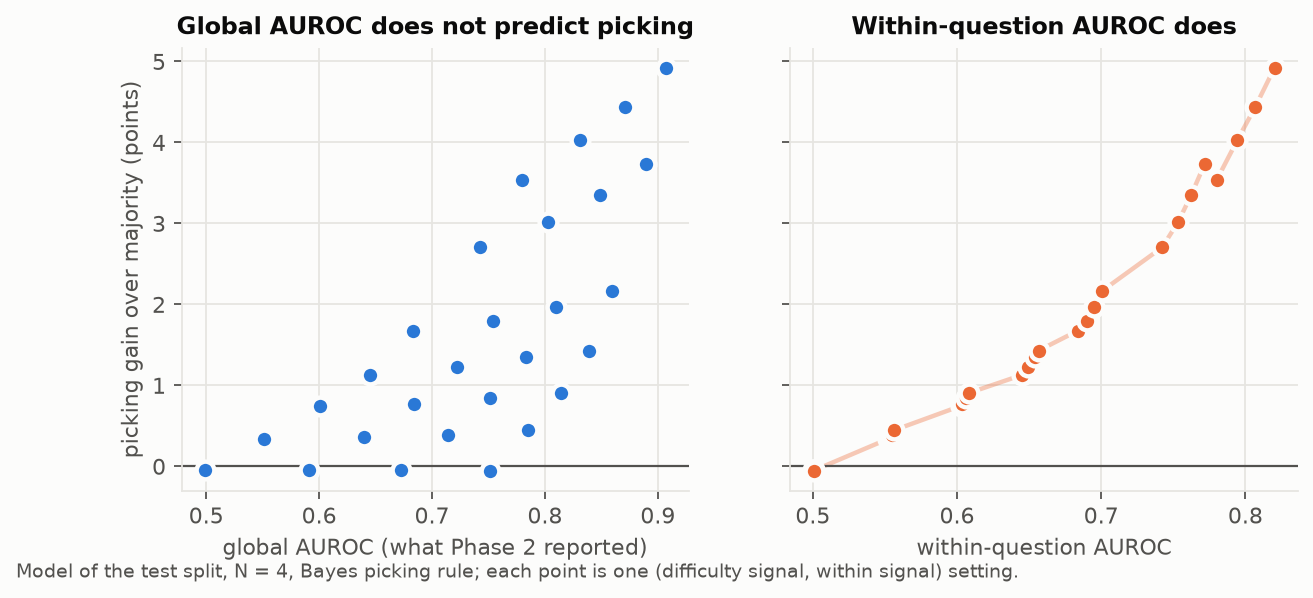
\includegraphics[width=\columnwidth]{figures/fig1_auroc_vs_gain.png}
\caption{Picking gain over majority vote in the calibrated model ($N=4$, Bayes rule). Left: against pooled AUROC.
Right: against within-question AUROC.}
\label{fig:auroc}
\end{figure}

\subsection{Most of the headroom is ties}
\label{sec:headroom}

At $N=4$ the 8.7-point gap between majority vote and pass@4 splits as follows:
\begin{itemize}
\item \textbf{Ties (5.7 points):} configurations such as (right, wrong, wrong, wrong) all different, where majority
  vote is a coin flip.
\item \textbf{Overturns (3.0 points):} the right answer has to beat a larger wrong group.
\end{itemize}

\paragraph{Proposition 1 (tie-breaking).}
Take majority vote and let the judge decide only among tied groups. If right scores are $\mathcal N(d,1)$ and wrong
scores $\mathcal N(0,1)$, independently, then
\begin{equation}
\begin{split}
\mathrm{gain}={}&P_{1\text{-}1\text{-}1\text{-}1}\Big(M_4(d)-\tfrac14\Big)\\
&+P_{2\text{-}2}\Big(\Phi(d)-\tfrac12\Big)\ \ge 0,
\end{split}
\end{equation}
where $M_4(d)=\int\phi(t-d)\Phi(t)^3\,dt$ and $P_{\cdot}$ are the configuration shares ($6.7\%$ and $1.3\%$ on
test). The closed form matches simulation to within $0.07$ points.

By contrast, Phase~2's summed-confidence rule can fall below majority vote: a single confident wrong attempt can
outscore two right ones.

Overturning a plurality of $m$ with a single right attempt under the Bayes rule (vote weight $\beta$) succeeds with
probability $\Phi\big([(1-m)\beta+(1+m)d^2/2]/(\sqrt{1+m}\,d)\big)$, which is small for weak judges.

The headroom also sits on hard questions: mean solve rate $0.33$, against $0.54$ for the pairs a within-question AUROC
averages over. We therefore report within-question AUROC on \emph{contested} questions, where majority vote does not
already pick the right answer.

\section{When Verification Pays}
\label{sec:scaling}

\paragraph{Majority vote saturates.}
As $N\to\infty$, majority vote is right on question $x$ if and only if $p_x$ exceeds the mass of every wrong answer;
in the model, iff $p_x>\rho(1-p_x)$. That probability is $78.3\%$ on the test calibration, while pass@$N\to100\%$.
Simulated majority accuracy reaches $77.7$, $78.2$ and $78.8$ at $N=8$, $16$ and $64$, a plateau also reported for
large-sample voting \citep{brown2024monkeys}.

\paragraph{Proposition 2 (aggregation is consistent, argmax is not).}
Score each answer group $C_a$ by $\sum_{i\in C_a}\log\Lambda(s_i)$, and suppose judge errors are conditionally
independent. Then the score divided by $N$ converges to
\[
\begin{gathered}
\pi(a)\,\mathrm{KL}(f_1\Vert f_0)>0 \text{ for the right answer},\\
-\pi(a)\,\mathrm{KL}(f_0\Vert f_1)<0 \text{ for a wrong one},
\end{gathered}
\]
so accuracy tends to $P(p_x>0)$ for \emph{any} judge with $d>0$. Picking the single top-scored attempt instead
converges to the precision of the top score bin, the imperfect-verifier ceiling of \citet{stroebl2026limits}.

If judge errors are shared within an answer group (correlation $\rho_s$), a right-versus-wrong group comparison is
capped at $\Phi(d/\sqrt{2\rho_s})$.

\paragraph{The compute crossover.}
Charge an attempt 1 unit and a judge verdict $0.3$. In the model, verification cannot beat majority vote at equal
compute for budgets of 8 units or fewer, even with within-question AUROC $0.78$. It wins only after majority vote
saturates: $+0.6$ to $+3.0$ points at 16 units and $+1.9$ to $+6.1$ at 32. Phase~2 tested picking at 4 attempts with
4 verdicts each, inside the region where verification must lose.

\paragraph{Contest-adaptive verification (CAV).}
These results suggest a simple procedure:
\begin{enumerate}
\item Sample 4 attempts. If all four give the same answer, stop: about $50\%$ of questions, right $99.4\%$ of the
  time in the model.
\item Otherwise sample up to $N_1$ attempts.
\item Judge only the attempts in the two largest answer groups, at most $m$ per group.
\item Pick the group maximising $n_g\,(\beta+\overline{\mathrm{logit}\,P(\text{correct})})$, where $n_g$ is the group
  size and $\beta$ is a vote weight tuned on development data.
\end{enumerate}
Adaptive stopping alone \citep{aggarwal2023adaptive} reaches the majority plateau with less compute, but cannot pass
it; only the judge can. In the model CAV gains $+1.7$ to $+5.3$ points over majority vote at equal average cost
($\approx11$ units). The gain holds when attractor strength varies across questions, when the judge is weaker on hard
questions, and when judge errors are shared within answer groups (Appendix~\ref{app:robust}).
Section~\ref{sec:stage1} tests CAV on the model's own attempts.

\section{Training a Judge for Selection}
\label{sec:training}

Outcome-labelled verdict training rewards a judge for predicting whether an attempt's answer is right.

On our pools, $56\%$ of the label entropy is question difficulty:
\[
H(Z)=0.91 \text{ bits} = \underbrace{I(Z;X)}_{0.51} + \underbrace{\mathbb E[H(p_x)]}_{0.40}.
\]
With 4 attempts per question, $53\%$ of wrong attempts come from questions with no right attempt. These carry no
within-question contrast. On a globally balanced set like Phase~2's, a judge that knows only $p_x$ earns $86\%$ verdict
reward.

\paragraph{Proposition 3 (pointwise--selection misalignment).}
Suppose the judge sees one attempt with a difficulty-like cue $x_b=s_b z_x+e_b$ that varies between attempts of the
same question (length, for example), and a within cue $x_w=dZ+e_w$. For a score $\theta_b x_b+\theta_w x_w$,
\begin{equation}
d'_{\text{within}}=d\,\theta_w/\sqrt{\theta_b^2+\theta_w^2}.
\end{equation}
\begin{itemize}
\item When $P(Z\mid x)$ varies with $x$, the pointwise-optimal $\theta_b$ is positive and strictly lowers
  within-question discrimination.
\item Class rebalancing changes only the intercept.
\item Under \emph{per-question balance} ($P(Z{=}1\mid x)=\frac12$ for every $x$), $x_b$ carries no information and
  $\theta_b=0$. The initial gradient on any question-only feature is then $\mathbb E[(\frac12-Z)\varphi(x)]=0$.
\end{itemize}

In a finite-sample learning model with 64-dimensional features, 900 questions and 1,024 training examples, per-question
balanced or pairwise data raise within-question AUROC from $0.67$ to $0.74$ while \emph{lowering} pooled AUROC from
$0.86$ to $0.74$ (Figure~\ref{fig:training}). Judge checkpoints must therefore be compared on within-question AUROC,
not pooled AUROC.

Per-question pairs scale as $N(N-1)\,\mathbb E[p(1-p)]$ per question: $1.07$ at $N=4$ and $21.4$ at $N=16$.

\begin{figure}[t]
\centering
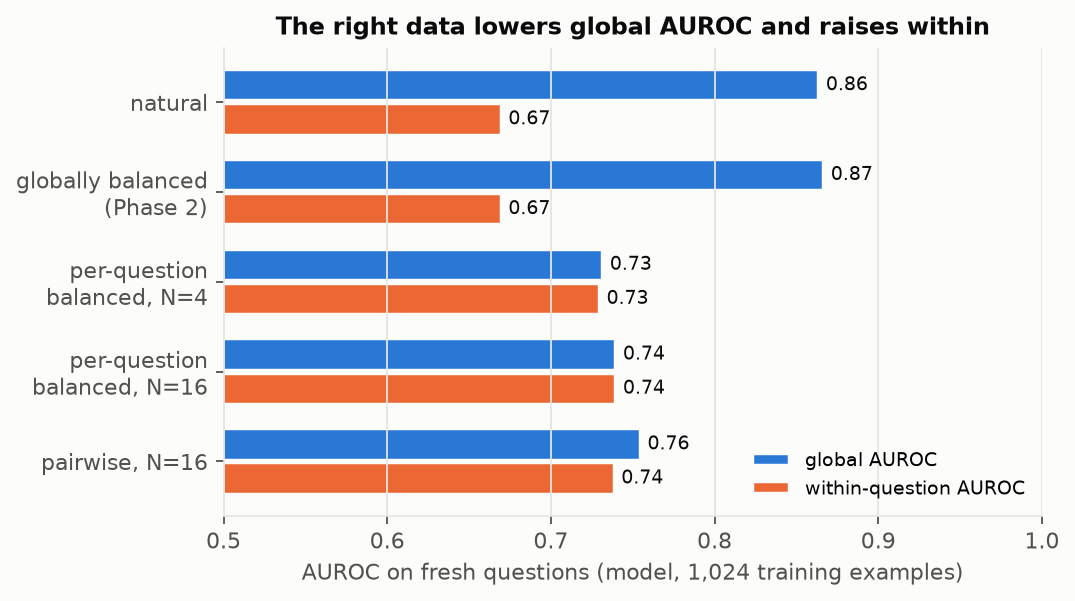
\includegraphics[width=\columnwidth]{figures/fig4_training_regimes.png}
\caption{Learning model (1,024 examples from 900 questions). Per-question balanced and pairwise data trade pooled
AUROC for within-question AUROC.}
\label{fig:training}
\end{figure}

\section{Experiments}
\label{sec:results}

We generate 16 attempts for each of 1,000 questions (dev 200, test 400, extra 400) with the mixed adapter, and judge
every answered attempt with the same adapter. All settings are tuned on dev and evaluated on test $\cup$ extra.

\paragraph{The pipeline reproduces Phase 2, and the model predicts the scaling curves.}
The Phase-3 pools match the Phase-2 numbers:
\begin{itemize}
\item \textbf{Dev:} single attempt $69.8\%$, pass@4 $86.3\%$, majority@4 $78.1\%$ (Phase~2: $69.8$, $86.5$, $77.5$).
\item \textbf{Test:} $67.0$, $82.8$, $74.9$ (Phase~2: $67.4$, $82.8$, $74.0$).
\end{itemize}
The model was fitted only to the Phase-2 4-attempt aggregates. On test it predicts majority@8 $=77.5$ (observed
$77.5$), majority@16 $=78.2$ (observed $78.7$) and pass@16 $=90.8$ (observed $90.2$). It also predicts the share of
4-attempt configurations where the majority is already right ($71.7\%$ vs $72.3\%$) and where no attempt is right
($17.2\%$ vs $17.3\%$).

Majority vote saturates at the predicted limit ($78.3\%$) while pass@16 reaches $90.2\%$ (Figure~\ref{fig:scaling}).
On test, adaptive-consistency reaches the same plateau ($78.7\%$) with fewer attempts but cannot pass it.

\paragraph{Judge-free features already reach the trained judge's pooled AUROC.}
Table~\ref{tab:trace} scores attempts by length, by counts of self-correction phrases, or by guess phrases.

\begin{itemize}
\item \textbf{Pooled:} these features reach AUROC 0.65--0.70, the level the Phase-2 trained self-judge reached
  (0.665). Hard questions produce long, hesitant attempts.
\item \textbf{Within question:} 0.54--0.61.
\item \textbf{Contested questions:} 0.46--0.58, about chance. This is where picking happens (\S\ref{sec:headroom}).
\end{itemize}

The table is the invariance theorem in miniature: a large pooled AUROC that selection cannot use.

The same data support the liveness account (Appendix~\ref{app:proofs}): $98$--$99\%$ of \emph{right} attempts contain
self-corrections, about 25 per attempt (36 per wrong attempt). A detector of ``an error occurred somewhere'' therefore
fires on almost every trace. What decides correctness is whether an error is still live at the end.

\begin{table*}[t]
\centering\small
\resizebox{\linewidth}{!}{\begin{tabular}{@{}llcccc@{}}
\toprule
Set & Trace feature & Pooled AUROC & Within-question & Contested within & Mean (right / wrong) \\
\midrule
dev & Length (tokens) & 0.700 & 0.580 & 0.495 & 7521.8 / 10005.3 \\
dev & Self-corrections (``wait'', ``actually'', \dots) & 0.677 & 0.563 & 0.477 & 23.8 / 34.9 \\
dev & Guess phrases (``let's assume'', \dots) & 0.680 & 0.611 & 0.577 & 1.0 / 2.4 \\
dev & Final-answer tags & 0.529 & 0.549 & 0.488 & 1.0 / 1.2 \\
test & Length (tokens) & 0.655 & 0.573 & 0.486 & 7977.9 / 9750.5 \\
test & Self-corrections (``wait'', ``actually'', \dots) & 0.648 & 0.553 & 0.514 & 26.0 / 36.0 \\
test & Guess phrases (``let's assume'', \dots) & 0.656 & 0.576 & 0.568 & 1.1 / 2.3 \\
test & Final-answer tags & 0.526 & 0.536 & 0.509 & 1.0 / 1.1 \\
\bottomrule
\end{tabular}}
\caption{Judge-free trace features. They reach the pooled AUROC of the Phase-2 trained self-judge (0.665) because hard questions produce long, hesitant attempts, but are near chance on contested questions, where picking happens. Almost every right attempt contains self-corrections.}
\label{tab:trace}
\end{table*}


\subsection{Stage 0: what the judge knows}
\label{sec:stage0}

Table~\ref{tab:stage0} tests the leniency account of \S\ref{sec:lenient} on test attempts 0--3, judged with four
chains each.

\begin{itemize}
\item \textbf{The judge is lenient.} It says ``incorrect'' to about one attempt in seven; $d'=0.49$.
\item \textbf{Sampled verdicts look near chance.} One verdict gives AUROC $0.57$; the share of four gives $0.64$.
\item \textbf{Probabilities recover the signal.} The verdict probability averaged over the four chains, and the
  direct probability read with no reasoning at all, reach $0.69$--$0.71$. That is the latent AUROC the model
  inferred from Phase-2 flag rates alone ($0.715$). Both paired differences from the four-verdict share are
  significant: $+0.067$ $[+0.047, +0.085]$ and $+0.090$ $[+0.049, +0.130]$ (paired bootstrap over questions).
\item \textbf{Verdicts on one attempt are strongly correlated.} Four ``incorrect'' verdicts on the same wrong attempt
  occur about $12\times$ as often as independent verdicts would allow. This is the persistent per-attempt component
  of Eq.~\ref{eq:judge}.
\end{itemize}

Within questions (Table~\ref{tab:pools}), the judge's discrimination is lower than pooled, and lowest on contested
questions, where the headroom lies. The verification signal is weakest where selection needs it: the configuration
analysis of \S\ref{sec:headroom} anticipated this.

\begin{table}[t]
\centering\small
\resizebox{\linewidth}{!}{\begin{tabular}{@{}lcc@{}}
\toprule
Test attempts 0--3, 4 chains each & Measured & Model \\
\midrule
Share of ``incorrect'' verdicts (sampled) & 0.154 & 0.04 (Phase 2 dev) \\
Hit rate $H$ / false-alarm rate $F$ & 0.255 / 0.125 & 0.074 / 0.022 \\
$d'=z(H)-z(F)$ & 0.49 & 0.57 \\
AUROC, 1 sampled verdict & 0.565 & 0.526 \\
AUROC, share of 4 sampled verdicts & 0.635 & 0.568 \\
AUROC, verdict probability, 1 chain & 0.689 & -- \\
AUROC, verdict probability, mean of 4 chains & 0.694 & $\le$0.715 \\
AUROC, direct probability (no reasoning) & 0.717 & -- \\
$P$(4 of 4 ``incorrect'' $\mid$ wrong), observed & 0.0422 & 0.005 \\
\quad same, if verdicts were independent & 0.00352 & 0.00003 \\
Chains reaching a verdict & 0.902 & 0.89 (Phase 2) \\
\bottomrule
\end{tabular}}
\caption{Stage 0: the untrained mixed judge on its own test attempts (1486 answered attempts, 28.7\% wrong). ``Model'' is the latent judge fitted to Phase-2 single-verdict flag rates (\S\ref{sec:lenient}).}
\label{tab:stage0}
\end{table}

\begin{table*}[t]
\centering\small
\resizebox{\linewidth}{!}{\begin{tabular}{@{}lcclccc@{}}
\toprule
Set & Single attempt & Score & Pooled AUROC & Within-question AUROC & Contested within-question AUROC \\
\midrule
dev & 0.698 & chain & 0.692 & 0.620 [0.578, 0.660] & 0.612 [0.508, 0.712] \\
 & & direct & 0.730 & 0.634 [0.576, 0.692] & 0.596 [0.460, 0.732] \\
 & & length & 0.699 & 0.580 [0.537, 0.623] & -- \\
test & 0.670 & chain & 0.682 & 0.611 [0.573, 0.645] & 0.511 [0.423, 0.604] \\
 & & direct & 0.718 & 0.614 [0.566, 0.658] & 0.469 [0.375, 0.575] \\
 & & length & 0.655 & 0.573 [0.541, 0.606] & -- \\
extra & 0.682 & chain & 0.713 & 0.668 [0.638, 0.700] & 0.631 [0.561, 0.703] \\
 & & direct & 0.746 & 0.661 [0.622, 0.699] & 0.641 [0.551, 0.731] \\
 & & length & 0.688 & 0.596 [0.568, 0.627] & -- \\
\bottomrule
\end{tabular}}
\caption{Judging own attempts (16 per question; first chain). ``Length'' scores an attempt by its token count. Brackets: 95\% question-cluster bootstrap intervals.}
\label{tab:pools}
\end{table*}


\subsection{Stage 1: contest-adaptive verification}
\label{sec:stage1}

\paragraph{Vote-only methods plateau.}
On test $\cup$ extra (800 questions), majority vote rises from $76.0\%$ at $N=4$ to $79.8\%$ at $N=16$, while
pass@16 is $91.4\%$. Adaptive-consistency reaches $79.8\%$ with $10.4$ attempts on average, and no threshold takes it
higher (Table~\ref{tab:selection}).

\paragraph{CAV passes the plateau (pre-registered primary test).}
CAV uses the chain probability with $N_1=16$, $m=8$ and $\beta$ tuned on dev. It reaches $81.0\%$ at an average cost
of $11.3$ units ($114$k decoded tokens per question). Against majority vote at the same cost ($79.4\%$) the
difference is $+1.6$ points $[+0.5, +2.6]$. At matched decoded tokens it is $+1.4$ $[+0.4, +2.5]$.

Against adaptive-consistency at the closest cost the difference is $+1.2$ $[+0.05, +2.3]$. CAV is also above
majority@16 ($79.8\%$) while using $29\%$ fewer units.

The size of the gain was predicted before any judging. Feeding the judge's dev within-question AUROC ($0.62$--$0.63$)
into the semi-synthetic model gave $\approx+1.3$ points.

Where does the gain come from? Classify each question by its 16-attempt answer distribution.
\begin{itemize}
\item \textbf{Right answer in the minority} ($10.6\%$ of questions): CAV gains $+11.1$ points on average, $+1.18$ of the
  total $+1.60$.
\item \textbf{Ties} ($1.8\%$): $+0.28$.
\item \textbf{Majority already right} ($79\%$): $+0.14$.
\item \textbf{No right attempt} ($8.6\%$): exactly $0$, as Theorem~1 requires.
\end{itemize}
At $N=16$, verification wins mainly by overturning wrong pluralities, not by breaking ties.

\begin{figure}[t]
\centering
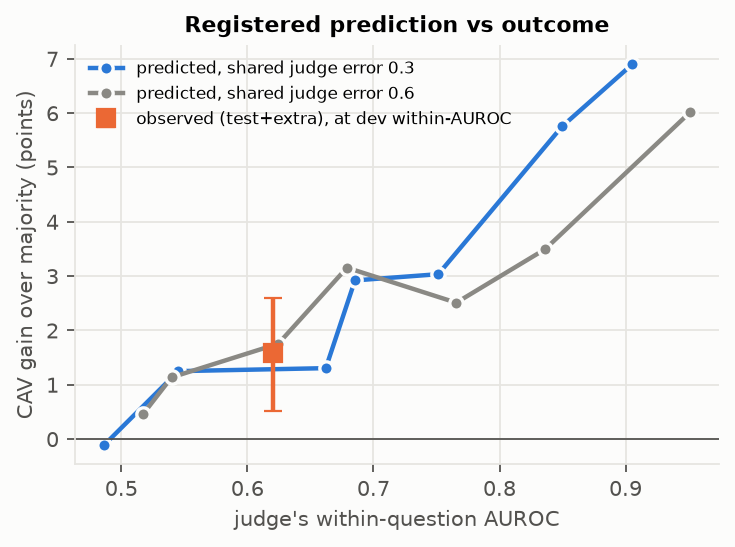
\includegraphics[width=\columnwidth]{figures/prediction_vs_outcome.png}
\caption{CAV gain as a function of the judge's within-question AUROC, predicted before any judging from the real dev
answer structure with simulated judges (lines). The square is the observed pre-registered result on test $\cup$ extra
(95\% CI), placed at the real judge's dev within-question AUROC.}
\label{fig:prediction}
\end{figure}

\paragraph{Cheap verification pays even at small budgets.}
CAV with the direct probability needs only a prefill pass per judged attempt. With $N_1=8$, $m=4$ it reaches
$79.2\%$ at $6.1$ units, $+1.3$ $[+0.8, +1.9]$ over majority vote at the same cost ($+1.3$ $[+0.8, +1.8]$ at matched
tokens). Adaptive-consistency is as good at that budget ($-0.5$ $[-1.2, +0.2]$).

The crossover of \S\ref{sec:scaling} assumed a verdict costs $0.3$ of an attempt. With prefill-only reads, it moves to
smaller budgets, as the cost term predicts.

\paragraph{Argmax is worse than voting; aggregation is not.}
Picking the single attempt with the best verdict probability gives $76.7\%$ at $N=16$, \emph{below} majority vote
($79.8\%$). Summing log-odds over answer groups gives $80.9\%$, as Proposition~2 predicts. CAV gets the aggregation
gain at about half the cost by judging only contested questions.

\paragraph{A learned combination raises AUROC but not picking.}
The exploratory combiner (fitted on dev) raises within-question AUROC on extra to $0.717$ (test $0.666$). It does not
improve CAV accuracy (Table~\ref{tab:selection}). Within-question AUROC averaged over all questions is the wrong
target: the gain has to come from contested questions, where the combiner is still near chance on test.

\begin{table}[t]
\centering\small
\resizebox{\linewidth}{!}{\begin{tabular}{@{}lcccc@{}}
\toprule
& Majority right & Tie & Overturn & Unwinnable \\
\midrule
dev & 0.749 & 0.066 & 0.050 & 0.135 \\
test & 0.723 & 0.062 & 0.042 & 0.173 \\
extra & 0.743 & 0.075 & 0.043 & 0.139 \\
model (test calibration) & 0.717 & 0.080 & 0.030 & 0.172 \\
\bottomrule
\end{tabular}}
\caption{Shares of 4-attempt configurations (random 4-subsets of the 16 attempts). Only ties and overturns can be won by a judge.}
\label{tab:configs}
\end{table}

\begin{table}[t]
\centering\small
\resizebox{\linewidth}{!}{\begin{tabular}{@{}lccc@{}}
\toprule
Rule & Acc. (\%) & Cost & Tokens \\
\midrule
Majority, $N=4$ & 76.0 & 4.00 & 35.7k \\
Majority, $N=8$ & 78.7 & 8.00 & 71.4k \\
Majority, $N=12$ & 79.5 & 12.00 & 107.1k \\
Majority, $N=16$ & 79.8 & 16.00 & 142.8k \\
pass@16 (oracle) & 91.4 & 16.00 & 142.8k \\
Adaptive-consistency, $t=0.8$ & 79.1 & 4.01 & 40.5k \\
Adaptive-consistency, $t=0.9$ & 79.7 & 6.41 & 64.0k \\
Adaptive-consistency, $t=0.99$ & 79.8 & 10.39 & 99.6k \\
Bayes aggregation, $N=4$ & 76.7 & 5.12 & 47.5k \\
Bayes aggregation, $N=16$ & 80.9 & 20.49 & 189.7k \\
Best-of-$N$ argmax, $N=4$ & 75.3 & 5.12 & 47.5k \\
Best-of-$N$ argmax, $N=16$ & 76.7 & 20.49 & 189.7k \\
CAV (chain), $N_1=8$, $m=4$ & 79.0 & 6.70 & 65.2k \\
CAV (direct), $N_1=8$, $m=4$ & 79.2 & 6.09 & 56.1k \\
CAV (combo-cheap), $N_1=8$, $m=4$ & 79.0 & 6.09 & 56.1k \\
CAV (direct), $N_1=12$, $m=4$ & 79.7 & 8.08 & 76.5k \\
CAV (chain), $N_1=12$, $m=8$ & 80.3 & 9.15 & 91.1k \\
CAV (direct), $N_1=16$, $m=4$ & 80.1 & 10.06 & 96.8k \\
CAV (chain), $N_1=16$, $m=8$$^\star$ & 81.0 & 11.31 & 113.9k \\
CAV (combo), $N_1=16$, $m=8$ & 79.6 & 11.31 & 113.9k \\
\bottomrule
\end{tabular}}
\caption{Selection on test $\cup$ extra (800 questions), settings tuned on dev. Cost: attempt $=1$, judge chain $=0.3$, direct read $=0.05$; tokens: decoded tokens per question. $^\star$: pre-registered primary rule.}
\label{tab:selection}
\end{table}


\begin{figure}[t]
\centering
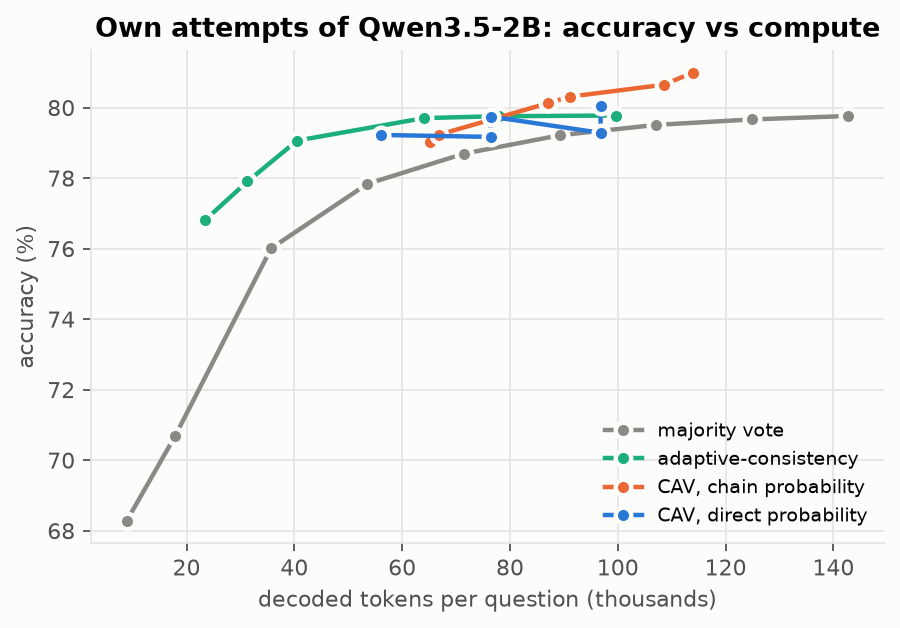
\includegraphics[width=\columnwidth]{figures/real_frontier.png}
\caption{Accuracy against decoded tokens per question on test $\cup$ extra (own attempts of Qwen3.5-2B). Settings
tuned on dev.}
\label{fig:frontier}
\end{figure}

\begin{figure*}[t]
\centering
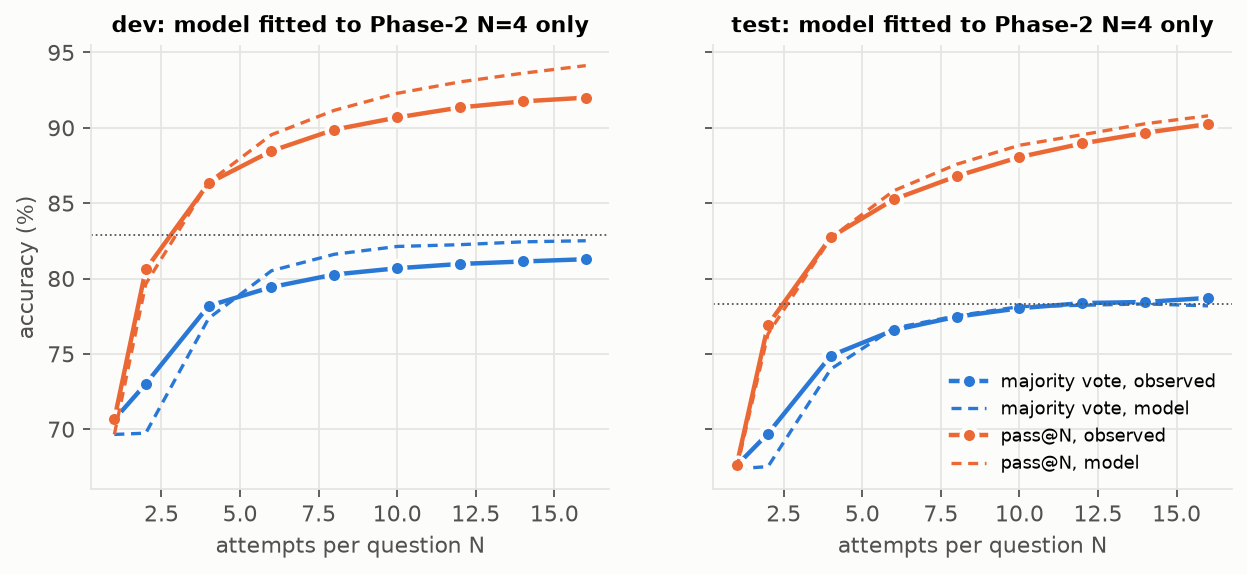
\includegraphics[width=0.8\textwidth]{figures/scaling_observed.png}
\caption{Majority@$N$ and pass@$N$ on own attempts (points) against the model fitted only to Phase-2 4-attempt
aggregates (dashed). Dotted line: the predicted majority limit $P(p_x>\rho(1-p_x))$.}
\label{fig:scaling}
\end{figure*}

\paragraph{Training the judge (future work).}
We also retrained the judge with the Phase-2 recipe in two arms: globally balanced, as in Phase~2, and per-question
balanced (Proposition~3). Verdict reward rose from $40\%$ to $57\%$ and from $48\%$ to $53\%$ respectively; the smaller
rise is consistent with the removed difficulty shortcut. We did not evaluate the trained judges on the selection pools,
so Proposition~3 rests on theory and the learning model of \S\ref{sec:training}.


\section{Related Work}
\label{sec:related}

\paragraph{Verifiers and selection.}
Outcome verifiers for best-of-$N$ \citep{cobbe2021gsm8k}, process supervision \citep{lightman2023verify} and step-level
benchmarks \citep{zheng2025processbench} measure verifier quality per solution. We instead measure what selection and
repair can use.

Weighted voting with log-odds weights is classical \citep{nitzan1982optimal,berend2014consistency}. Combinations of
weak verifiers \citep{saadfalcon2025weaver} and resampling limits under imperfect verifiers \citep{stroebl2026limits}
bound what verification can add. Compute-optimal test-time scaling \citep{snell2024scaling}, adaptive stopping for
self-consistency \citep{wang2023selfconsistency,aggarwal2023adaptive} and scaling models of voting systems
\citep{chen2024morecalls,brown2024monkeys} motivate our compute-matched comparisons.

\paragraph{Explaining aggregate behaviour with per-problem heterogeneity.}
\citet{schaeffer2025monkeys} explain power-law scaling of repeated sampling with a heavy-tailed distribution of
per-problem success rates. Our Beta-distributed solve rates play the same role for verification.

\paragraph{Self-verification and its limits.}
Self-correction without external feedback often fails \citep{huang2024cannot,stechly2025selfverification}.
\citet{song2025mindthegap} formalise a generation--verification gap that governs self-improvement. Our governing
quantity is within-question discrimination on contested questions.

\citet{bulut2026problem} show that pooled probe AUROCs can come entirely from difficulty. We extend this to verifiers
used for selection and repair, where it becomes an invariance theorem. Signal-detection analyses of LLM judges
separate sensitivity from criterion \citep{sdt2026signal}. We show that verdict sampling turns a lenient criterion into
a near-chance AUROC.

\section{Limitations and Conclusion}
\label{sec:conclusion}

\paragraph{Limitations.}
\begin{itemize}
\item We study one solver family at 2B parameters and one judge (the same adapter).
\item Labels come from an answer checker, so an attempt with flawed reasoning and a right answer counts as right.
\item The step conversion of attempts is our own: Phase~2's converter was lost.
\item The CAV gain is modest ($+1.6$ points) because the judge's discrimination on contested questions is weak.
\item The length and liveness mechanisms (Appendix~\ref{app:proofs}) predict judging degrades with length and
  self-corrections. Within the 4k--16k-token range of our attempts we see no such degradation; only the premise that
  almost every right trace contains self-corrections is confirmed.
\item Costs are counted in units and decoded tokens, not wall-clock time.
\end{itemize}

\paragraph{Conclusion.}
How good a self-verifier looks depends on what is measured.
\begin{itemize}
\item Sampled verdicts hide a lenient judge's signal: probabilities recover $0.07$--$0.09$ AUROC.
\item Pooled AUROC rewards knowing which questions are hard. Trace features alone match a trained judge pooled and are
  at chance where picking happens.
\item Small-$N$ picking puts verification where it cannot win.
\end{itemize}
A small model of these effects, fitted to 4-attempt aggregates, predicts 16-attempt behaviour to within a point.
Measured within questions, scored by probability, and spent only on contested questions after self-consistency
saturates, a 2B model's judgement of its own work beats compute-matched majority vote and adaptive-consistency.

\bibliography{references}

\appendix

\section{Proofs}
\label{app:proofs}

\paragraph{Pair-share identity.}
A pooled AUROC averages $\mathbb 1[s_w>s_r]$ (ties $\frac12$) over all wrong--right pairs. Partitioning the
$K(QN-K)$ pairs into the $\sum_x k_x(N-k_x)$ same-question pairs and the rest gives the stated convex combination.
For the expectation, use $\mathbb E[k_x(N-k_x)]=N(N-1)\,\mathbb E[p(1-p)]$ and $K\approx QN\bar p$.

\paragraph{Theorem 1.}
\emph{Repair.} A fresh draw for question $x$ is right with probability $p_x$, so replacing attempt $i$ changes
expected accuracy by $p_x-Z_i$, and a flag $f_i$ contributes $f_i(p_x-Z_i)$. Since
$\mathbb E[Z\mid x]=p_x$,
\[
\mathbb E[f(p_x-Z)\mid x]=-\mathrm{Cov}(f,Z\mid x).
\]
If $f$ depends only on $x$, this covariance is $0$.

The optimal flag sets $f=1$ exactly when $\mathbb E[p_x-Z\mid x,s]>0$, that is, when $P(Z{=}1\mid x,s)<p_x$.

\emph{Selection.} Given the answers and the scores, the posterior that answer group $C_a$ is right is proportional to
$\pi(\text{answers}\mid a\text{ right})\prod_{i\in C_a}f_1(s_i\mid x)\prod_{i\notin C_a}f_0(s_i\mid x)$. Dividing by
$\prod_i f_0(s_i\mid x)$ leaves $\pi(\cdot)\prod_{i\in C_a}\Lambda_x(s_i)$. If $f_1=f_0$ given $x$, then
$\Lambda\equiv1$ and only the vote pattern remains. $\square$

\paragraph{Proposition 1.}
Majority vote and the lexicographic rule differ only in tied configurations.
\begin{itemize}
\item \emph{Four singletons, one of them right:} the rule is right iff the right attempt has the top score, with
  probability $M_4(d)=\int\phi(t-d)\Phi(t)^3dt$, against $\frac14$ for a random tie-break.
\item \emph{Two groups of two:} the rule compares group means, which differ by $\mathcal N(d,1)$, so it is right with
  probability $\Phi(d)$, against $\frac12$.
\end{itemize}
Both increments are non-negative for $d\ge0$.

\paragraph{Overturn probability.}
Write the log-likelihood ratio of a score as $\ell(s)=ds-d^2/2$. Then $\ell$ is $\mathcal N(d^2/2,d^2)$ for a right
attempt and $\mathcal N(-d^2/2,d^2)$ for a wrong one. For a right group of size $k$ against a wrong group of size $m$,
the score difference is
\[
\begin{gathered}
(k-m)\beta+\textstyle\sum_{C}\ell-\sum_{W}\ell\\
\sim\ \mathcal N\big((k-m)\beta+(k+m)d^2/2,\ (k+m)d^2\big).
\end{gathered}
\]

\paragraph{Proposition 2.}
By the law of large numbers, $\frac1N\sum_{i\in C_a}\ell_i\to\pi(a)\,\mathbb E[\ell\mid Z_a]$, with
$\mathbb E[\ell\mid Z{=}1]=\mathrm{KL}(f_1\Vert f_0)$ and $\mathbb E[\ell\mid Z{=}0]=-\mathrm{KL}(f_0\Vert f_1)$.

With group-shared noise of correlation $\rho_s$, a group mean keeps variance $\rho_s+(1-\rho_s)/n\to\rho_s$, which gives
the stated cap.

For argmax with scores quantised to $V$ verdicts, the top bin is reached with positive probability by both right and
wrong attempts. The rule therefore converges to $P(Z{=}1\mid\text{top bin})$.

\paragraph{Proposition 3.}
Within a question $z_x$ is constant, so a right and a wrong attempt differ in score by $\theta_w d$ plus noise of
variance $2(\theta_b^2+\theta_w^2)$.

Under per-question balance, $x_b$ is independent of $Z$ given $x$, and also marginally, since $P(Z\mid x)=\frac12$.
The pointwise-optimal weight on it is therefore zero. At initialisation, the logistic gradient on any feature
$\varphi(x)$ is $\mathbb E[(\sigma(0)-Z)\varphi(x)]=\mathbb E[(\frac12-\frac12)\varphi(x)]=0$.

\paragraph{Length law.}
Suppose step scores are Gumbel and $m$ of $T$ steps are shifted by $\log L$. The maximum of independent Gumbels with
locations $\mu_i$ is Gumbel with location $\log\sum_ie^{\mu_i}$, and two independent Gumbels compare logistically.
Hence the solution-level AUROC of a max-pooled detector is
\[
\frac{T-m+mL}{2T-m+mL}.
\]
A step-level AUROC of $0.80$ ($L=4$) gives $0.51$--$0.53$ at $T=100$--$200$, the level of the hidden-state error
feature on own attempts in Phase~2.

\section{Robustness of CAV in the model}
\label{app:robust}

\begin{table}[h]
\centering\small
\begin{tabular}{@{}lcc@{}}
\toprule
Scenario & $d=0.5$ & $d=1.0$ \\
\midrule
Baseline ($\rho$ constant, $\rho_s=0.3$) & +2.4 & +5.3 \\
Judge weaker on hard questions & +1.8 & +4.2 \\
Shared judge errors, $\rho_s=0.6$ & +1.7 & +4.1 \\
Variable attractor strength & +1.8 to +2.2 & +3.1 to +4.1 \\
\bottomrule
\end{tabular}
\caption{CAV ($N_1=16$, $m=8$, probability scoring) minus majority vote at equal average cost ($\approx11$ units), in
points, in the calibrated model.}
\end{table}

\section{Experimental details}
\label{app:details}

\paragraph{Question sets.}
\begin{itemize}
\item \emph{test}: the 400-question FINAL-v3 SOLVE test split.
\item \emph{dev}: the 200-question development slice used in Phase~2, used here only for tuning.
\item \emph{extra}: 400 SOLVE training questions that no run of the mixed adapter could have seen (all 1,134 SOLVE
  questions of its GRPO manifest and the trial slices are excluded).
\item \emph{train}: 450 further such questions for Stage 2.
\end{itemize}
Sets are fixed by a seeded script before any generation.

\paragraph{Sampling.}
Attempts use the SOLVE prompt with temperature $1.0$, no top-$p$/top-$k$ truncation and a 16,384-token cap. An attempt is
correct if it finishes, passes the strict format gates and its last final-answer tag matches the key under the
project's rule-based checker. Answers are grouped by checker equivalence.

\paragraph{Judging.}
Each answered attempt is split into steps: paragraphs, with display maths and very short paragraphs merged into the
previous step, plus a final step ``The final answer is $X$''. The judge prompt is the v2 JUDGE prompt.
\begin{itemize}
\item A reasoning chain (temperature $1.0$, 8,192-token cap) stops at ``Decision:''.
\item The verdict probability is read from the top-20 next-token log-probabilities after appending ``Decision:'',
  taking the first of up to four forced positions that shows a verdict token. Chains that were cut off or never
  reached the label get a probability too.
\item The \emph{direct} probability appends ``Decision:'' right after the prompt, with no reasoning.
\item Test attempts 0--3 get four chains each; all other attempts one.
\end{itemize}

\paragraph{Costs and statistics.}
Unit costs (pre-registered): attempt $=1$, chain $=0.3$, direct read $=0.05$ (added after the smoke test). Decoded-token
costs count attempt and chain tokens and exclude prefill. Every rule is averaged over 100 random orders of each
question's 16 attempts. Majority at a fractional cost mixes the two neighbouring $N$. 95\% intervals use 1,000--2,000
bootstrap resamples of questions; within-question AUROCs are bootstrapped over questions (cluster bootstrap).

\paragraph{Pre-registration.}
\texttt{phase3/PREREGISTRATION.md} fixed the sets, sampling, judging, primary rule, primary comparison and success
criterion before any attempt was generated. It also records three deviations and the semi-synthetic gain predictions
made before any judging, each with its hash.


\end{document}
